\documentclass[12pt,fleqn]{article}
\setlength{\parindent}{0pt}
\usepackage{graphicx}
\usepackage{listings}
\usepackage[latin5]{inputenc}
\setlength{\parskip}{8pt}
\setlength{\parsep}{0pt}
\setlength{\headsep}{0pt}
\setlength{\topskip}{0pt}
\setlength{\topmargin}{0pt}
\setlength{\topsep}{0pt}
\setlength{\partopsep}{0pt}
\setlength{\mathindent}{0cm}

\begin{document}
MIT OCW Cok Degiskenli Calculus - Ders 13

Lagrange Carpanlari (Multipliers)

Amac $f(x,y,z)$ gibi birden fazla degisken iceren bir fonksiyonu maksimize
etmek, degisik olan, $x,y,z$ degiskenlerinin birbirinden bagimsiz
ol\textbf{ma}masi. Bu degiskenlerin arasindaki iliski $g(x,y,z)=c$ gibi bir
fonksiyon tarafindan gosteriliyor olabilir, $c$ bir sabittir. Yani
$f(x,y,z)$'i minimize ya da maksimize ediyoruz ve bunu sadece $g(x,y,z)=c$
sartina / sinirlama ifadesine (constraint) uyan $x,y,z$ degerleri icin yapiyoruz.

Bunun icin hangi teknigi kullaniriz? Yollardan biri, eger sinirlama ifadesi
basit ise, belki bir degiskeni cebirsel olarak cozebiliriz (digerleri
baglaminda ifade ederek), sonra geri $f$'e sokariz, boylece klasik bir min
/ maks problemi elde ederiz, ki o tur bir problemi cozmeyi artik biliyoruz.

Fakat bazen $x,y,z$ degiskenleri icin analitik cozum mumkun olmaz, o zaman
farkli teknikler kullanmamiz gerekir. Bu derste ogrenecegimiz teknikler
bunlar olacak. 

Uygulama baglaminda, Lagrange Carpanlari bize niye ilgilendiriyor? Belki
fizik, termodinamik dersinde gormussunuzdur, sicaklik, hacim ve basinc
degerleri vardir, ve bu degerler birbirinden bagimsiz
degildir. Termodinamikte $pv = nrt$ denklemi vardir, gerci burada analitik
olarak basitlestirme yapabilirdik, ama bazi sartlarda tum degiskenleri
oldugu gibi tutmayi isteyebiliriz. 

Simdiye kadar min / maks problemleri icin gordugumuz kritik nokta bulma
tekniklerinin burada ise yarayamacagini hemen belirtelim. O kritik noktalar
$g(x,y,z)=c$ sinirlama ifadesini tatmin etmiyor olabilirler. Baska bir seye
ihtiyacimiz var. 

Ornek

Hiperbol $xy =3$ uzerinde olan ve orijine en yakin noktayi bul. 

Aslinda bu soruyu temel geometri kullanarak cozebiliriz, fakat burada
Lagrange Carpanlari kullanarak cozecegiz, cunku iyi bir ornek. 

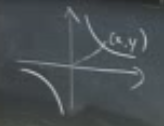
\includegraphics[height=2cm]{13_1.png}

Neyi minimize edelim? Mesela $f(x,y) = \sqrt{x^2 + y^2}$ olur mu? Olabilir,
ama karekok ifadesinden kurtulursak daha iyi olur. 

O zaman

\[ min \ f(x,y) = x^2 + y^2 \]

\[ ki, \ xy = 3  \]

Yani sinirlama ifadesi $g(x,y) = xy$ olarak sectik. 

Grafige bakalim. Yuvarlaklar $f(x,y)$ konturlari, yesil okla gosterilen
mesela $f(x,y) = 20$ konturu. Bu kontur ust sag kose ve sol alt kosede
gosterilen hiperbolu kesiyor mu? Evet. Fakat $f(x,y) = 10$, vs. diyerek
daha kucuk yuvarlaklar elde edebilir miyim? Evet. Fakat bir noktadan sonra
bu halkalar hiperbolu kesmeyecektir. 

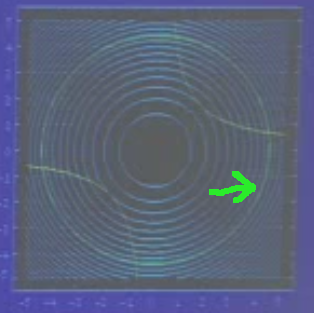
\includegraphics[height=4cm]{13_2.png}

Aradigimiz $x,y$ degerleri hiperbole teget olan, olabilecek en kucuk
yuvarlak.

Cozum icin tegetlik kavramindan faydalanabiliriz. Eger olabilecek en
minimal $f$, her iki fonksiyonun kesit egrilerinin teget oldugu noktada
ise, bu noktayi bulmaya ugrasabilirim. 

Iki kesit egrisi birbirine teget ise, onlarin teget duzlemi paraleldir,
eger oyleyse, bu duzlemlerin normalleri birbirine paralel olmalidir. 

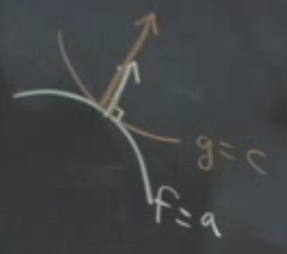
\includegraphics[height=4cm]{13_3.png}

Bu normallerin ayni boyda olmasi gerekmez, yukaridaki gibi, ama paralel
olmalari gerekir. Bu durumda 

\[ \nabla f // \nabla g \]

ifadesi dogru olmalidir, yani $f$'in gradyani $g$'nin gradyanina
paraleldir. Bazi ornekler

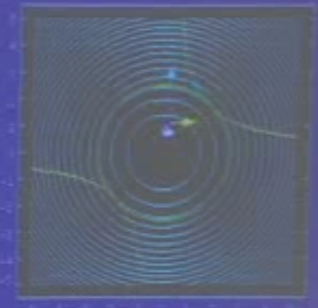
\includegraphics[height=3cm]{13_4.png}

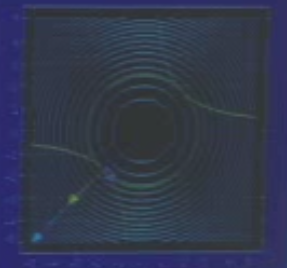
\includegraphics[height=3cm]{13_6.png}

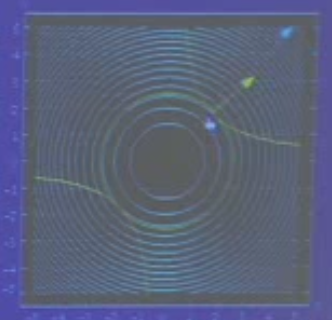
\includegraphics[height=3cm]{13_5.png}

Goruldugu gibi minimal noktalarin birinde (ustteki son resim) gradyanlar
paralel. 

Cebirsel olarak dusunursek: vektorler ne zaman birbirine paralel olur?
Birbirlerinin kati olduklari zaman. Yani su sekilde bir ifadeyi
yazabildigimiz zaman

\[ \nabla f = \lambda \nabla g \]

ki $\lambda$ bir sabit. 

Gradyanlar ayni yonu gostermiyor olabilir, bu durumu $\lambda$'nin negatif
olup olmamasi halledecektir.

Yani aradigimiz $xy$ uzerinde sayisal deger $\lambda$ uzerinden $\nabla f =
\lambda \nabla g $ 
ifadesinin dogru oldugu bir nokta, ve $\lambda$ degeri
ariyoruz (unutmayalim, gradyanlar belli $x,y$ degerleri uzerinden
alinir). Yani 2 degisken iceren sinirlama ifadesi $g(x,y)=c$ iceren bir min /
maks problemi yerine, bir denklem sistemi geciriyoruz. Bu sistem nedir?
Yani ustteki gradyan formuludur, o da su sisteme donusur:

\[ f_x = \lambda g_x \]

\[ f_y = \lambda g_y \]

Oyle degil mi? Cunku $\nabla f$ ve $\nabla g$ birer vektordur, 

\[ 
\nabla f =
\left[\begin{array}{r}
f_x \\
f_y
\end{array}\right], \ \ 
\nabla g =
\left[\begin{array}{r}
g_x \\
g_y
\end{array}\right]
 \]

O zaman iki ustteki denklem sistemi suradan ileri gelmektedir

\[ 
\left[\begin{array}{r}
f_x \\
f_y
\end{array}\right]  = 
\lambda
\left[\begin{array}{r}
g_x \\
g_y
\end{array}\right]
 \]

Fakat hala eksik bir sey var. Elimizde $x,y,\lambda$ bilinmeyenleri var,
ama sadece iki tane formul var. Eksik olan $g(x,y) = c$, cunku $x,y$
birbirinden bagimsiz degil ve $g$ uzerinden baglantililar. Simdi oldu. 3
formul soyle:

\[ f_x = \lambda g_x \]

\[ f_y = \lambda g_y \]

\[ g(x,y) = c \]

Ornegimiz 

\[ f(x,y) = x^2 + y^2 \]

\[ g(x,y) = xy  \]

uzerinde uygularsak

\[ 2x = \lambda y \]

\[ 2y = \lambda x \]

\[ xy = 3 \]

Bu sistemi cozmemiz gerekiyor. Yanliz sunu soyleyelim, bu sistemi cozmenin
genel (hep isleyen) bir yontemi yoktur. Cozum bazen cok basittir, bazen
zordur, bazen sadece sayisal / numerik / hesapsal acidan cozulebilir
(bilgisayar ile). Bu ornekte kolay. 

\[ 2x - \lambda y = 0\]

\[ 2y= \lambda x = 0 \]

\[ xy = 3 \]

Matris formuna koyarsak

\[ 
\left[\begin{array}{rr}
2 & -\lambda \\
\lambda & -2
\end{array}\right]
\left[\begin{array}{r}
x \\ y
\end{array}\right]
=
\left[\begin{array}{r}
0 \\ 0
\end{array}\right]
 \]

En basit cozum $x=0,y=0$ sinirlama ifadesi $xy=3$'u cozmez. Diger cozum ne
zaman ortaya cikar? Eger matrisin determinanti sifir ise. 

\[ 
\left|\begin{array}{rr}
2 & -\lambda \\
\lambda & -2
\end{array}\right| = -4 + \lambda^2 = 0
 \]

\[ <=> \lambda^2 = 4 \]

\[ <=> \lambda = \pm 2 \]

Elimizde iki durum var. $\lambda$ ya 2, ya da -2. 

1. $\lambda = 2$ durumunda

\[ x = y \]

\[ x^2 = 3 \]

O zaman

$(x,y)$ = $(\sqrt{3}, \sqrt{3})$ ya da $(-\sqrt{3}, -\sqrt{3})$ 

2. $\lambda = -2$ durumunda

\[ x = -y \]

\[ -x^2 = 3 \]

Bu durumda cozum yoktur (karesi alinip eksi ile carpilan hicbir sayi 3
sonucunu vermez). 

Ustteki son iki resime bakinca, $\lambda = 2$'nin dogru oldugunu goruyoruz,
cozum olan iki noktada bir gradyan otekinin hakikaten tam iki kati. 











\end{document}
